\chapter{具体需求}

\section{功能需求}
ETS考试与管理系统可以分为两个子系统,分别供考生用户使用和ETS管理人员使用。对于面向考生的系统,其主要包括以下功能:

1、新用户注册;

2、注册用户查询个人登记信息;

3、注册用户查询考场信息;

4、注册用户预缴费;

5、注册用户报名考试;

6、已参加考试的用户查询成绩。

对于面向ETS管理人员的系统,其主要包括以下功能:

1、ETS发布考试场次信息;

2、ETS进行题库维护;

3、ETS发布成型试题;

4、ETS分发试卷进行考试;

5、ETS进行试卷批改。

\subsection{新用户注册}

\subsubsection{介绍}
本功能接受用户输入的注册信息,包括姓名、地区、邮寄地址、联系方式等,要求用户设置一个密码,并为该用户生成一个唯一的ID。对用户提交的不符合要求的注册信息的处理方式是拒绝生成新账户并要求用户重新填写。新账户创建成功后,在用户数据库中为之关联一条记录,其中包括了账户余额、已报名考试等信息。

\subsubsection{输入}
以下信息为用户必填:

1、姓:由大小写英文字母组成的字符串,长度不超过50

2、名:由大小写英文字母组成的字符串,长度不超过50

3、身份证号:符合身份证号的国家规定

4、性别:从男或女中选择

5、生日:从所给年、月、日菜单中选择

6、地区:从菜单中所给的国家/地区中选择

7、邮寄地址:国家、城市从菜单中选择,街道地址是长度不超过100的字符串

8、联系方式:分手机和邮箱,其中手机号必须是加区号的数字,区号从菜单中选择

以下信息为用户选填:

1、中文姓名:

2、称呼:Mr/Ms/Mrs/Miss

\subsubsection{处理}
系统接收到数据后,首先按照上述约束进行注册信息的有效性检测。如果用户未填写某些必填信息,或所填信息不合要求,例如查询不到用户输入的身份证号,将拒绝生成新账户,并告知用户发生错误。

若用户所填信息完整无误,则进入下一步,要求用户为账户设定一个密码,密码的规范是必须由英文字母或数字组成,至少6位。

以上步骤完成后,弹出界面要求用户确认所有填写的信息已完整无误,并提供两个按键:若用户需修改信息,则按返回键,否则按确认键。用户按下确认键后,即在数据库中添加一条账户记录。

在生成账户之前的以上各步骤中,若遇到不可抗干扰(如网络中断等),系统将自动撤销所有临时记录,并停止创建账户。用户再次创建账户必须重启整个过程。

\subsubsection{输出}
用户创建账户成功后,即可根据ID和密码登录个人中心,登录后可以进行后续的查询考试信息、缴费等操作。

\subsection{个人信息查询与修改}

\subsubsection{介绍}
本功能适用于已注册用户。用户登录个人中心后,将看到分成几个部分的操作选项,其中一部分名为“个人资料”,包括更新联系信息和修改密码两个操作。更新联系信息指的是更新用户在注册账户时填写的信息,不包含多余信息,也不缺少任何信息。

\subsubsection{输入}
更新联系信息的界面与注册时输入联系信息的界面类似,此时各个项的默认值是用户上次保存的值。只要满足3.1.1部分说明的约束,用户可以任意修改个人信息。修改完成后,点击“取消”将撤销本次修改并恢复到上次保存的值,点击“确认”将保存本次修改。

修改密码时,首先要求用户能正确输入原来的密码,否则拒绝此操作。当用户正确输入原来的密码后,让用户输入新的密码,并再次输入以便确认。完成后,密码就已修改。

\subsubsection{处理}
在处理更新联系信息操作时,当用户点击“确认”后,系统将对收到的信息进行检查,以确认所填信息满足要求。检查未通过时,拒绝更新信息并告知用户发生错误。检查通过后,修改数据库中该用户的信息。

在处理修改密码操作时,共有两个动作,一是检查用户输入的原密码是否正确,如果不正确就拒绝操作。二是将合法的新密码写入数据库替代旧密码。

\subsubsection{输出}
该功能没有显式输出,它的结果就是数据库中用户的记录得到了更新。

\subsection{查询考试信息}

\subsubsection{介绍}
该功能是系统的主要功能之一,用户可以在这里查询到一年内的考点与场次信息,主要包括考试的时间、地点和剩余考位。

用户登录系统后,在个人中心的考试信息一栏,可以点击“全年考试时间与地点查询”或“考位查询”,后者返回的信息比前者更具体,包括某个考点某场次各个考场的剩余考位。

\subsubsection{输入}
“全年考试时间与地点查询”没有输入。

“考位查询”要求用户指定考场和场次,查询的时间范围是从当前时刻开始往后12个月,因为查询已结束的场次的考位信息没有意义。

\subsubsection{处理}
系统收到查询请求后,从数据库中取出所需数据。如果用户查询的是“全年考试时间与地点查询”,则取出一张事先存放的包括了所有考场全年场次安排的表返回给用户。如果用户查询的是“考位查询”,则要求用户从列表中选择一个考点和一个场次,然后从数据库中取出该考点该场次的所有考场的考位信息返回给用户。

\subsubsection{输出}
对于“全年考试时间与地点查询”,返回给用户的输出是一张表,每一条对应一个考点的考场号、地点与全年考试时间安排。
对于“考位查询”,返回给用户的是用户指定的某个考点、某个时间的所有考场的剩余考位数。

\subsection{预缴费}

\subsubsection{介绍}
用户使用本功能对账户进行充值,才能进行后续的考试报名等操作。用户缴纳的费用以人名币计,最小单位是1元,账户余额上限是9999元。若缴纳的费用超过限制,此次操作将被拒绝。用户可以点击“我的余额”,然后进行查询当前账户剩余金额、缴纳费用或申请退款等操作。

\subsubsection{输入}
接受的用户输入是充值金额与支付方式。
充值金额:默认单位是人名币,单笔充值金额上限是9999元。
支付方式:可选择各大银行的e支付、支付宝、微信支付

\subsubsection{处理}
系统接受到用户通过第三方支付机构支付的金额后,检查账户累计余额是否超过上限,如果未超过,就更新账户余额,否则将金额返还给用户,并告知余额超限。

\subsubsection{输出}
用户所缴费用加上原来的账户余额后得到当前余额,写入数据库中。用户缴费成功后,将可以在“我的余额”中看到账户余额已发生变化。

\subsection{考试报名}

\subsubsection{介绍}
本功能是考生用户子系统中最重要的功能之一,考生通过它进行考试报名。

\subsubsection{输入}
考生用户报名考试前,首先要指定要报名的考试类型,是TOFEL、GRE、GMAT的哪一个。用户必须确保自己账户余额足够支付该次考试的费用,否则报名将失败。然后,系统将提供给用户考试时间和考点的选择,时间范围是未来12个月,考点范围是全国范围内的考点。用户选择完毕后,进一步提供给用户该考点该场次各个考场的剩余考位情况,用户可以选择一个有剩余考位的考场报名考试。报名完成后,相应考试费用即从用户账户余额中扣除。

虽然每次点击“考试报名”链接只能进行一次考试报名,但用户可以多次报名,所有已报名但还未进行的考试都可以在“查看已注册考试”中查询到。

系统用于确保参加考试的考生身份的方式就是考生注册时填写的身份证号。

\subsubsection{处理}
系统接受到考试报名请求时,按如下步骤进行处理:

1、首先询问用户希望报名的考试类型。根据用户选择的考试类型与用户的当前账户余额,系统判断用户是否可支付此次考试的费用。如果不能,系统将告知用户报名失败,并提示用户先缴费再报名。如果可以,进入下一步。

2、系统提供给用户未来12月全国范围内所有考点的场次,供用户选择。待用户选择完时间和考点后,系统查询数据库中该考点该场次的考位信息,将还有剩余考位的考场信息返回给用户。

3、最后,用户选择一个考场,点击“确认”,系统收到确认信息后,显示“报名成功”,并向数据库中添加记录。之后,用户可以在“查看已注册考试”板块查询到这次的报名信息。

\subsubsection{输出}
用户成功报名一次考试后,系统在数据库中添加若干记录,包括在所有用户信息的表中增添该用户的已报名考试记录,在考试记录表中增添一条与该考场、该场次、该用户关联的信息。

最后,用户将在“查询已注册考试”板块查询到已报名的考试的具体信息,包括考场号、考试时间地点、参加考试人员的姓名、用于身份验证的证件号等。

\subsection{查看已注册考试}

\subsubsection{介绍}
本功能模块主要的作用有两个,一是供用户查询或确认已报名的考试,二是提供了更改考试时间、考场,申请缓考以及取消报名的操作。如果用户需要更改考试时间、考场,申请缓考、取消报名等操作,都必须在该场考试时间的24小时前完成。

\subsubsection{输入}
考生用户点击“查看已注册考试”链接后,即可查询到所有已报名但还未进行的考试的详细信息,包括考试类型、报名时间、考试时间、考场号、考生姓名、证件号等。用户可以一一检查确认无误。

在每一条考试信息下方,系统提供了“更改考试时间、考场”“申请缓考”“取消报名”三个按键。

如果用户点击“更改考试时间、考场”,系统无需进行账户余额的检查,而是直接提供给用户未来12月内全国所有考点的选择。用户选择完毕后,在数据库中更新相应记录。

“申请缓考”的操作是类似地,不同之处在于“申请缓考”不允许更改考场,用户可以选择在同一考点后续的场次进行考试。如果用户只是想推迟考试时间,用这个操作比较方便。

“取消报名”则是彻底删除本次报名信息并得到退款。

\subsubsection{处理}
用户点击“查看已注册考试”后,系统即从数据库中取出该用户的所有已报名考试信息返回给用户。

如果用户点击了某一条考试信息的“更改考试时间、考场”链接,则与考试报名时类似,系统提供给用户未来12月内全国所有考点的选择,接着提供有剩余考位的考场的选择。用户选择完毕确认后,数据库中的记录就得到更新。

如果用户点击“申请缓考”,系统告知用户该考点在未来6个月内所有场次及剩余考位的信息,供用户选择。用户选择完毕确认后,数据库中的记录就得到更新。

如果用户点击“取消报名”,系统弹出提示框,询问用户是否确定此操作。一旦用户确定,就将本考试报名信息从数据库中删除,并将退款写入用户账户余额。

\subsubsection{输出}
用户点击“查看已注册考试”后,数据库没有修改,前端界面展示给用户的是分条列出的所有已注册考试信息。

如果用户继续点击“更改考试时间、考场”“申请缓考”“取消报名”等链接,系统将更新数据库中的内容,用户再次进入“查看已注册考试”界面时,将看到信息已被修改。

\subsection{成绩查询}

\subsubsection{介绍}
本功能模块允许考生用户查询已参加考试的成绩、生成电子版成绩单、寄送成绩单、放弃成绩等。

\subsubsection{输入}
用户点击“成绩查询”后,系统将返回该用户参加的历次考试的成绩信息。对每一条成绩,用户可以选择“生成电子版成绩单”“寄送成绩单”和“放弃成绩”。

“生成电子版成绩单”无需额外的输入。

“寄送成绩单”需用户填写收件人、单位、地址。其中收件人中英文均可,不超过20个字符,单位名称中英文均可,不超过50个字符。地址分国家、城市、街道地址,国家和城市从系统提供的下拉菜单中选择,街道地址手动填写,不超过50个字符。

“放弃成绩”同样无需额外输入。

\subsubsection{处理}
系统从数据库中取出该用户所有已参加考试的成绩信息返回给用户。

如果用户点击了某条成绩信息的“生成电子版成绩单”,系统生成一份pdf格式的成绩单供用户下载。

如果用户点击了某条成绩信息的“寄送成绩单”,系统将要求用户填写收件人、单位名称、寄件地址。用户填写完毕确认后,系统自动扣除一笔寄件费用。如果账户余额不足将停止此次操作并提示用户缴费。如果扣款成功,将成绩单的寄送信息以某种方式提供给ETS负责寄送成绩单的管理人员。

如果用户点击了某条成绩信息的“放弃成绩”,系统将弹出提示框,询问用户是否确认此操作。如果用户确认,将本次考试成绩从数据库中删除。该操作是不可恢复的。

\subsubsection{输出}
用户点击“成绩查询”后,系统不对数据库作修改,查询用户的所有考试成绩后返回给用户。

如果用户继续点击“生成电子版成绩单”,系统生成该次考试成绩单的pdf版,供用户下载。

如果用户继续点击“寄送成绩单”,系统将以某种形式输出到服务器端,提示ETS管理人员有新的寄送成绩单任务。

如果用户继续点击“放弃成绩”,系统将删除数据库中的内容,用户再次进入“成绩查询”界面时,将看到成绩已被删除。

\subsection{题库维护}

\subsubsection{介绍}
本功能接受由管理人员输入的不同类型的题目,将其分别存储在数据库中。除此之外, 本系统允许管理人员依据需求增加或者删除对应的题目,根据已有的考试信息对部分题目标定难度,以及对题目的可能出现范围做出标定(例如,设置某些题目作为固定的加试题)。

\subsubsection{输入}
在登入本系统时,本系统应要求考场管理人员输入对应的账户名以及密码。确认登陆成功之后,以下信息可以作为有效的输入:

A. 管理人员提出增添某一类题目的要求。确认该要求后,题库维护系统需要要求管理人员输入以下内容

1、增添内容所对应的考试科目:TOEFL,GRE,GMAT等;

2、增添内容的具体类型:例如在TOEFL考试中,增添的题目具体属于听力、口语、阅读或者写作的哪一部分;

3、增添内容的标题:用于检索该部分内容;

4、增添内容的关键字(可选):用于搜索相关内容;

5、增添内容对应的考试材料:例如若内容对应与TOEFL的阅读部分,那么此部分将要求管理人员输入对应的文章;

6、增添内容所对应的题目:例如若内容对应TOEFL的阅读部分,那么管理人员将被要求输入某篇阅读所对应的所有题目。题目的类型应该从题库指定的内容中选择,例如双选题,多选题或者六选三;题目的数量和种类将依据增添内容的具体类型做出限定,例如在TOEFL阅读中必须出现一道六选三题目,单篇阅读所对应的题目数量不超过十四道且不少于十三道等。

以上内容应该要求管理人员按序依次输入。输入的内容的难度默认设置为1,类型设置为1;类型和难度的详细说明可以参见后文。

B. 管理人员提出删除/修改某一类题目的要求。确认该要求后,题库维护系统需要要求管理人员输入以下内容

1、删除/修改内容所对应的考试科目:TOEFL,GRE,GMAT等;

2、删除/修改内容的具体类型:例如在TOEFL考试中,增添的题目具体属于听力、口语、阅读或者写作的哪一部分;

3、删除/修改内容所含有的关键字(可选):某篇题目所对应的关键字;

4、删除/修改部分的标题(二选一,同下):所删除部分对应的标题;

5、删除/修改部分的编号(二选一,同上):在完成某一内容的增添后,数据库系统将为该内容生成一个唯一的编号。管理人员输入该编号,即可检索对应的内容。

以上内容应要求管理人员按序依次输入。在完成输入之后,系统将能够确定所要删除/修改的具体内容。之后,系统将要求管理人员输入以下内容:

1、删除/修改选项:管理人员将被要求输入具体选项(删除或者修改)。

2、如果管理人员输入删除选项,那么系统将询问管理人员所删除的具体题目,亦或是删除整个片段。选择完成之后应再次要求管理人员作出确定。

3、如果管理人员输入修改选项,那么对应的材料或者题目将进入可编辑状态,管理人员可以增加或者删除部分内容。这一部分的输入应该满足上文中增添内容所对应的题目中的约束。

C. 管理人员为某一类题目标定难度。确认该要求后,题库维护系统需要要求管理人员输入以下内容:

1、标定内容所对应的考试科目:TOEFL,GRE,GMAT等;

2、标定内容的具体类型:例如在TOEFL考试中,增添的题目具体属于听力、口语、阅读或者写作的哪一部分;

3、标定内容所含有的关键字(可选):某篇题目所对应的关键字;

4、标定部分的标题(二选一,同下):所标定部分对应的标题;

5、标定部分的编号(二选一,同上):在完成某一内容的增添后,数据库系统将为该内容生成一个唯一的编号。管理人员输入该编号,即可检索对应的内容。

以上内容应要求管理人员按序依次输入。在完成输入之后,系统将能够确定所要标定的具体内容。之后,系统将会要求管理人员输入一个难度系数值,这个值为整形值,且必须小于100大于零。

D. 管理人员为某一类题目设置类型。确认该要求后,题库维护系统应该要求管理人员输入以下内容:

1、标定内容所对应的考试科目:TOEFL,GRE,GMAT等;

2、标定内容的具体类型:例如在TOEFL考试中,增添的题目具体属于听力、口语、阅读或者写作的哪一部分;

3、标定内容所含有的关键字(可选):某篇题目所对应的关键字;

4、标定部分的标题(二选一,同下):所标定部分对应的标题;

5、标定部分的编号(二选一,同上):在完成某一内容的增添后,数据库系统将为该内容生成一个唯一的编号。管理人员输入该编号,即可检索对应的内容。

以上内容应要求管理人员按序依次输入。在完成输入之后,系统将能够确定所要标定的具体内容。之后,管理人员将被要求选择该部分内容所对应的模式。模式共有四种,用一个整形数表示,意义分别叙述如下:

1、该题目是正常类型的题目,可以出现在试题中,对应模式1;

2、该题目只可以出现在加试中,对应模式2;

3、该题目不能出现在试题中,对应模式3。

E. 管理人员需要查看某一类题目。题库管理系统将允许管理人员输入内容所对应的具体科目,内容对应的编号/关键字/标题,定义同上。
	
\subsubsection{处理}
在得到对应的输入之后,题库维护系统将做出如下处理:

A. 在管理人员的增添题目需求输入完成之后,题库维护系统将把管理人员输入的具体内容添加到数据库的表项中。数据库表的详细设计可在详细设计中查看,此处不展开。之后,数据库系统将为这部分内容生成一个唯一的内容编号,并且将内容编号以及其对应的关键字,标题和所属部分的具体信息添加到索引中,方便之后根据标题以及关键字进行检索。

B. 在管理人员删除题目的需求输入完成之后,题库维护系统将根据管理人员输入的内容在索引中寻找到正确的内容编号,并且根据输入做出如下判定:

1、如果输入要求删除整个内容,那么该内容所对应的材料和所有子题目都应该被删除。系统将清除该编号对应的材料和所有子题目,并且在索引中也删除该内容;

2、如果输入要求删除某一内容下的子题目,那么只有该子题目对应的表项会被删除。

C. 在管理人员修改题目的需求输入完成之后,题库维护系统将根据管理人员输入的内容在索引中寻找到正确的内容编号,并且根据输入做出以下判定:

1、如果管理人员需要修改某一内容所对应的材料,那么该部分将变为可编辑状态;

2、如果管理人员需要修改某一内容所对应的子题目,那么这一题目所对应的部分将变为可编辑状态。

之后,题库维护系统将再次根据输入更新被修改内容所对应的具体表项。

D. 管理人员为某一类题目修改难度的需求输入完成之后,题库维护系统将根据管理人员输入的内容在索引中寻找到正确的内容编号,并且将该内容对应的难度改为输入值。

E. 管理人员为某一类题目设置类型的需求输入完成之后,题库维护系统将根据管理人员输入的内容在索引中寻找到正确的内容编号,并且将该内容对应的类型改为输入值。

F. 管理人员为查看某一类题目的需求输入完成之后,题库维护系统将根据管理人员输入的内容在索引中寻找到正确的内容编号。

对于可能发生的异常情况,进行如下规定:

A. 如果根据管理人员输入的内容无法在索引中寻找到正确选项,那么系统将展示出错信息“无法寻找到指定的内容”,同时当前操作无效。

B. 如果管理人员在删除某一内容对应的子题目并且确认保存之后,该部分内容所包含的子题目数量或者内容不符合约束要求,那么系统将展示出错信息“该部分所对应的题目数量、类型不符合要求”,同时当前操作无效。

其余异常状态不做具体规定。

\subsubsection{输出}
待处理完成之后,题库维护系统将展示如下输出:

A. 当增添、修改、删除、设置内容类型及难度操作完成之后,题库维护系统将在屏幕上展示操作成功信息,并且重新显示初始菜单;

B. 当输入出现错误以及发生异常时,题库维护系统需要以弹窗或者浮动信息的方式在屏幕上展示出错信息;

C. 当系统根据输入在索引中查询到选项后,系统将在屏幕上展示检索到的内容所对应的具体标题,内容以及题目编号。


\subsection{试题成型}

\subsubsection{介绍}
本系统允许管理人设置题目信息以及题目难度,根据给定的题目难度和试题信息自动从题库中选择相应的题目拼成一套完整的试卷。本系统每次所抽取的题目数量及题目类型也应该能够人为进行设置;除此之外,本系统还有一些其他功能,例如上次抽取过的试题在一定时间之内不应该再次出现等。

\subsubsection{输入}
在登入本系统时,需要管理人员提供账号和密码,这里的账号和密码和之前的题库维护系统应该使用同一个数据库。在确认输入的账号密码有效后,以下信息可以作为有效的输入:

A. 管理人员提出出一套新试卷的要求。确认该要求后,试题成型系统将允许管理人员输入以下参数值:

1、题目难度阈值:接受输入为两个32位整形数,且必须均为正值,分别代表上限和下限。其中,下限值应该小于上限;

2、需要出题的具体考试科目:TOEFL,GRE,GMAT等。

接受以上参数之后,系统应该能够自动生成一套题目,其结果将会展示在屏幕上。之后,系统允许管理员做出以下输入:

1、修改其中部分题目的内容的要求。系统将会允许管理员输入需要修改的具体题目,之后管理人员将被允许从试题管理系统中重新选择该部分所对应的其他题目来替换当前题目;

2、确认生成结果的要求。一旦确认,系统将要求管理人员输入该部分题目所对应的考试时间。

B. 修改部分设置选项的要求。确认该要求后,试题成型系统将允许管理人员输入以下内容:

1、某一科目所对应难度阈值的缺省值:接受输入为两个32位整形数,且必须均为正值,分别代表上限和下限。其中,下限值应该小于上限;

2、某一科目所对应题目的类型和数量的缺省值:这里将允许管理人员输入具体科目题目类型和题目数量,例如托福的阅读部分默认包括3篇阅读,听力部分默认包含两个section等;

3、题目被重复利用的最小时间:这个值将保证一次题目被重复利用的时间差不小于该值。管理人员将输入一个时间长度值作为有效输入。

\subsubsection{处理}
根据不同的输入请求,系统将作出如下处理:

A. 接受管理人员出一套新试卷的要求之后,该系统将进入题库维护系统检索某一科目所对应的题目。系统将根据一个随机值随机地选择部分题目内容,检测该部分题目是否符合时间要求,若符合则将该部分编号添加到当前维护表内;之后重复以上过程,若题目编号重复丢弃当前选择重新置随机数,直到表项中的题目数量符合要求,或者题库维护系统中所有该类型对应题目都在表项中。之后,系统将把当前表内所有题目的难度系数值累加作为当前试卷的难度系数值;如果难度系数值不在范围内,那么系统将清空所维护的表,重新进行选择过程,直至结果符合要求,或者尝试次数超过上限。

B. 接受管理人员修改部分选项的要求之后,系统将管理人员的输入值覆盖当前设置文件内的已有值。

C. 管理人员确定生成结果之后,系统将把管理人员的所设置的时间戳与当前已有的时间戳进行对比,确认没有重复,并且时间戳在合法范围内。之后,该部分题目将被添加对应的时间戳,并且当前的生成的题目表将会被系统保存。

对于可能出现的异常情况,系统将做出如下处理:

A. 题库维护系统内所含有的所有题目都已将在当前所生成的试卷内,但是本套试卷所含有的题目种类或数量仍然不符合要求。此时将报错“题库维护系统内没有足够的题目”,并且取消当前请求;

B. 系统在给定的尝试次数内无法生成难度符合要求的题目,此时将报错“无法生成给定难度要求的题目”,并且取消当前请求;

C. 管理人员给某一次的考试重复生成了试卷,此时将报错“考试时间与已有时间重复”,并提醒管理人员修改时间戳。

其他异常情况不做具体规定。

\subsubsection{输出}
当处理完成之后,系统将展示如下输出:

A. 试卷生成成功之后,系统需要将当前试卷内容展示在屏幕上。

B. 管理人员完成了关于生成试卷部分所有的输入后,系统将以弹窗或者浮动信息的方式在屏幕上显示“(某时间)所对应的(某科目)的试卷已添加到数据库”;

C. 管理人员在提出修改部分设置选项的要求之后,系统需要将当前所有的设置选项展示在屏幕上供管理人员选择。


\subsection{试卷分发及测试}

\subsubsection{介绍}
本系统允许考生进行身份信息验证,并且提供一个可以操作的终端界面供考生进行考试。本系统将自动与题库维护及试题成型系统进行通讯,获取所需要的信息,并且将考生的考试结果通过内部网络传回至服务器。
	
\subsubsection{输入}
本系统首先要求考生完成身份验证。在考生完成身份验证之后,本系统将要求考场管理人员输入对应的管理密码。确认无误之后,本次考试将开始,本系统将允许考生输入对应题目的答案。对于不同的考试科目,对应的终端系统将有所不同。下面以TOEFL考试为例,对考试系统所拥有的终端界面以及输入做具体说明:

A. 对于阅读部分,考生可以做出如下有效输入:选择某一题目的答案,切换到上一题,切换到下一题,查看考试系统的使用帮助,确认完成阅读部分,隐藏以及显示时间等。

B. 对于听力部分,考生可以做出如下有效输入:开始当前的section,选择某一题目的答案,切换到下一题,查看考试系统的使用帮助,确认完成听力部分,隐藏及显示时间等。

C. 对于口语部分,考生可以做出如下有效输入:开始当前的口语部分,输入口语设备的测试用例,输入口语部分所对应的录音内容,查看考试系统的使用帮助等。

D. 对于作文部分,考生可以做出如下有效输入:开始当前的作文部分,输入作文部分的结果,切换到下一题,查看考试系统的使用帮助,确认完成作文部分,隐藏及显示时间等。

其余科目的考试系统输入将根据不同科目的具体要求而有所不同,此处不一一列举。

\subsubsection{处理}
本系统将根据考生的输入内容做出如下不同的处理。同样以TOEFL考试的考试系统为例,系统所进行的处理如下:

A. 在考生输入身份验证信息(照片以及身份证号)之后,系统将把考生的编号与系统内本次参与考试考生的身份信息进行对比。如果存在则返回合法值,否则将提示身份验证失败;

B. 在管理人员输入管理密码之后,考试系统将对考试管理人员的身份进行确认。如果比对结果一致,那么考试将开始,将提示身份验证信息失败;

C. 本次考试开始之后,考试系统将向远端服务器请求当前考试的题目内容。之后,远端服务器上的题库管理系统将从中取出对应的题目,并通过内部网络传回给考生所使用的考试系统。

D. 当考试的某一部分开始之后,该部分所对应的计时将启动;

E. 当考生完成了对某一题目的选择之后,该题目所对应的选项将被添加到考试结果所对应的表内。同样地,考生所作答的结果音频以及作文的文本内容也将被保存在本地数据库的表内;

F. 一旦考生确认完成试题的某一部分,或者该部分的时间已经耗尽之后,该部分的作答结果将被上传至远端服务器中,考试系统的终端界面将会切换到下一部分。

除此之外,对于TOEFL考试,还有以下附加需求:

加试需求:当考生开始某一部分(例如听力)之后,代表开始的信号将会被发送给远端服务器。远端服务器将产生一个随机值来决定此部分内容是否需要加试,如果需要则返回加试题目以及对应的题目编号,并发送给考试系统。考试系统将把加试题目随机插入到现有的题目中,并开始这一部分的测试;

\subsubsection{输出}
考试系统所输出的结果将作为终端界面的元素展示在终端上,具体有如下需求:

A. 在考生输入身份验证信息之后,考生的身份验证信息应该能够显示在屏幕上,以便于进一步确认是否正确;

B. 每一部分的开始之前,考生需要点击continue来确认开始本部分。continue选项需要显示在屏幕上。

C. 某一部分开始之后,终端界面需要能够展示该部分对应的题目和材料,以及在右上角显示上一题/下一题按钮。除此之外,终端界面需要在右上角显示该部分所对应的时间,并且提供一个按钮以便考生隐藏时间。另外,当当前部分剩余时间小于五分钟的时候,时间应该会被强制显示并闪动以便提醒考生。除此之外,对于每一部分所展示的内容应该不同,例如听力部分需要显示音量调节按钮;

D. 当考试点击显示帮助内容的按钮之后,终端将显示帮助内容。

E. 当每一部分完成之后,终端将以弹窗或者浮动窗口的形式展示该部分已完成的信息。

F. (可选)在整个过程中,用户端将应该在醒目位置展示ETS的logo。

\subsection{试卷批改}

\subsubsection{介绍}
本系统将对之前在测试系统中收集到的考生测试信息进行汇总和统计,并且对考生的答案进行批改并生成最终分数。对于机器可以批改的题目,本系统将会自动地将考生的答案与标准答案进行匹配,并生成考生的分数;对于机器无法批阅的题目,本系统将把考生的答案以易于查阅的方式展现给阅卷人员,并且自动统计分数以生成考生的最终成绩。除此之外,本系统还拥有对考生成绩进行分析的功能,用于评估试卷难度和改进出题方向。

\subsubsection{输入}
本系统接受考生的试卷答案作为输入。同时,阅卷人员将能够通过输入账号和密码登入系统;系统确认账号和密码匹配之后,以下信息可以作为有效的输入:

A. 阅卷人员需要批改的科目:TOEFL,GRE,GMAT等;

B. 阅卷人员需要批改的具体题目:如对于TOEFL考试,阅卷人员可以选择批改作文或者口语部分。

确认阅卷人员的输入选择之后,阅卷人员可以查阅考考生的答案,并且将分数作为有效地输入。分数为一双精度浮点数,对分数的具体限制依考试科目和具体的题目类型而有所不同。

除此之外,试卷批改系统的管理人员也能够通过不同的账号和密码登入系统;系统确认账号和密码匹配之后,以下信息可以作为有效的输入:

A. 管理人员请求在系统中新建一个阅卷人员账号:管理人员将被要求输入阅卷人员的用户名,密码以及该阅卷人员有权限批改的具体科目;

B. 管理人员请求查看某一场考试的统计信息:管理人员将把某一场考试所对应的具体科目和场次(或者时间)作为有效输入。

C. 管理人员请求对阅卷人员的账号信息作出修改:管理人员将输入一个账号名称,之后他将被要求输入新的密码和批改权限。

\subsubsection{处理}
考试系统接受输入后,所做出的处理具体如下:

A. 考试系统接受考生的答案之后,考试系统将对考生的答案进行分类,并且将可以由机器批改的题目(例如选择题)与标准答案进行匹配,生成考生该部分的最终分数。对于不能由机器进行批改的题目,系统也将对其归类,并且将其最终分数留空等待阅卷人员填入;

B. 考试系统接受阅卷人员的阅卷请求之后,考试系统首先将检查该阅卷人员是否具有此部分的批阅权限,如果没有,考试系统将报错。否则,考试系统将从数据库中随机选择对应部分某考生批阅未达指定次数的题目,并且将此题目的考生答案中反馈给阅卷人员。得到阅卷人员的批阅分数之后,考试系统将该分数存入对应的表内;当某考生的题目批阅已经到达指定次数时,系统将计算所有阅卷人员的平均分数作为考生本题的最终得分。

C. 考试系统接受管理人员的新建账号和修改账号请求时,系统会根据管理人员的具体输入更新账号管理所用的数据库表。当考试系统接受管理人员查看某一场考试统计信息的时候,系统将判断该场考试是否所有考生的信息都已经被批阅完毕;如果是,那么系统将展示所有考生各部分的平均分、标准差、中位数、最低及最高分数以及其他可用的统计信息。

\subsubsection{输出}
考试系统可以将如下部分作为有效的输出:

A. 考试系统待阅卷人员选择具体的科目及题目类型之后,考试系统将随机选择的考生答案以易于阅读的方式展现在屏幕上,并且展现一个输入框供试卷批改人员输入分数;

B. 考试系统接受管理人员展示该场考试统计信息的要求之后,考试系统将把相关的信息以易于阅读的方式展现在屏幕上;

C. 对于相关的报错信息以及提示,该系统将把报错信息以弹窗或者浮动信息的方式展现在屏幕上;

D. 当某一次考试所有的考生试卷都已经批阅完毕后,考生的成绩信息应该能够交付给成绩查询系统。

\section{性能需求}

\subsection{系统响应时间要求}
根据业务管理分析,本系统采用数据集中管理方式作为系统开发的基础。

考生使用的子系统,主要包括创建账户、浏览个人信息、缴费、考试报名、成绩查询等功能,用户通过浏览器上网访问系统。因此,系统对用户操作的响应时间将受网络速度的影响。对响应时间的要求是在1M/s网速下,正常情况下1s内返回用户请求的数据,峰值情况下10s内返回用户请求的数据。

ETS管理人员使用的子系统,主要包括发布考试场次信息、题库维护、试题成型部分,用户可以直接在服务器端访问系统。因此,系统对用户的响应时间主要取决于存储器读写速率,这部分对响应时间的要求是在500M/s的磁盘读写速率下,5min内完成对整套试题大小的数据的读写。

\subsection{系统安全性要求}
1、数据要绝对安全防止有意无意的破坏数据。若数据遭到破坏,系统具有数据恢复功能,不可恢复的数据仅限于修改后未保存的数据。系统需定期备份;

2、考生用户只有通过客户端所提供的各功能接口访问数据库,ETS管理员可以在服务器端通过服务器端子系统管理数据库;

3、ETS方面在更新数据库中的所有活动,如更新考试安排信息、更新成绩等,必须有主管进行审核,并做好记录;

4、系统本身需具备抵御攻击的能力,不存在严重漏洞。

\subsection{可靠性}
1、要能够抵御用户可能的误操作,保证系统的健壮性;

2、要对考生填写的数据或ETS管理员发布的数据进行完整性检验,保证数据有效性;

3、通过备份等方式,使得在数据被破坏时,具有数据恢复能力。

\subsection{易使用性}
1、无论是提供给考生的浏览器显示界面,还是提供给ETS管理员的系统管理界面,系统各种操作提示清晰、含义明确,可方便使用者进行操作;

2、重要信息显示在明显的地方,使使用者可清楚的了解到信息;

3、信息录入尽量使用选择,避免填写大量信息而造成不一致性。

\subsection{并发性}
系统对并发性的需求主要来自需同时支持大量的考生用户访问。预期系统应当支持每秒千次的考生用户访问请求,支持同时使用的用户数目为100000。

由于每个考生用户只能读写与自己账户关联的数据,因此可以在本软件系统层面支持多考生用户同时的查询、修改请求。(当进入到操作系统层面时,对文件系统的读写请求可能采取不同的方案)。但由于ETS管理员使用的子系统具有对数据的更大的操作权限,因此不允许两个服务器端子系统同时对数据库进行写操作。

\subsection{稳定工作时间}
在正常的工作量下,系统应当能长时间持续稳定运行。

在峰值工作量下,系统应当能稳定运行至少24小时。

\section{外部接口需求}

\subsection{用户接口}
\subsection{1层数据流图}

A. 对于用户注册与管理系统的用户接口说明如下,这一部分对应于功能需求中新用户注册、个人信息查询与修改、查询考试信息以及预缴费的部分:

\begin{figure}[ht]
\centering
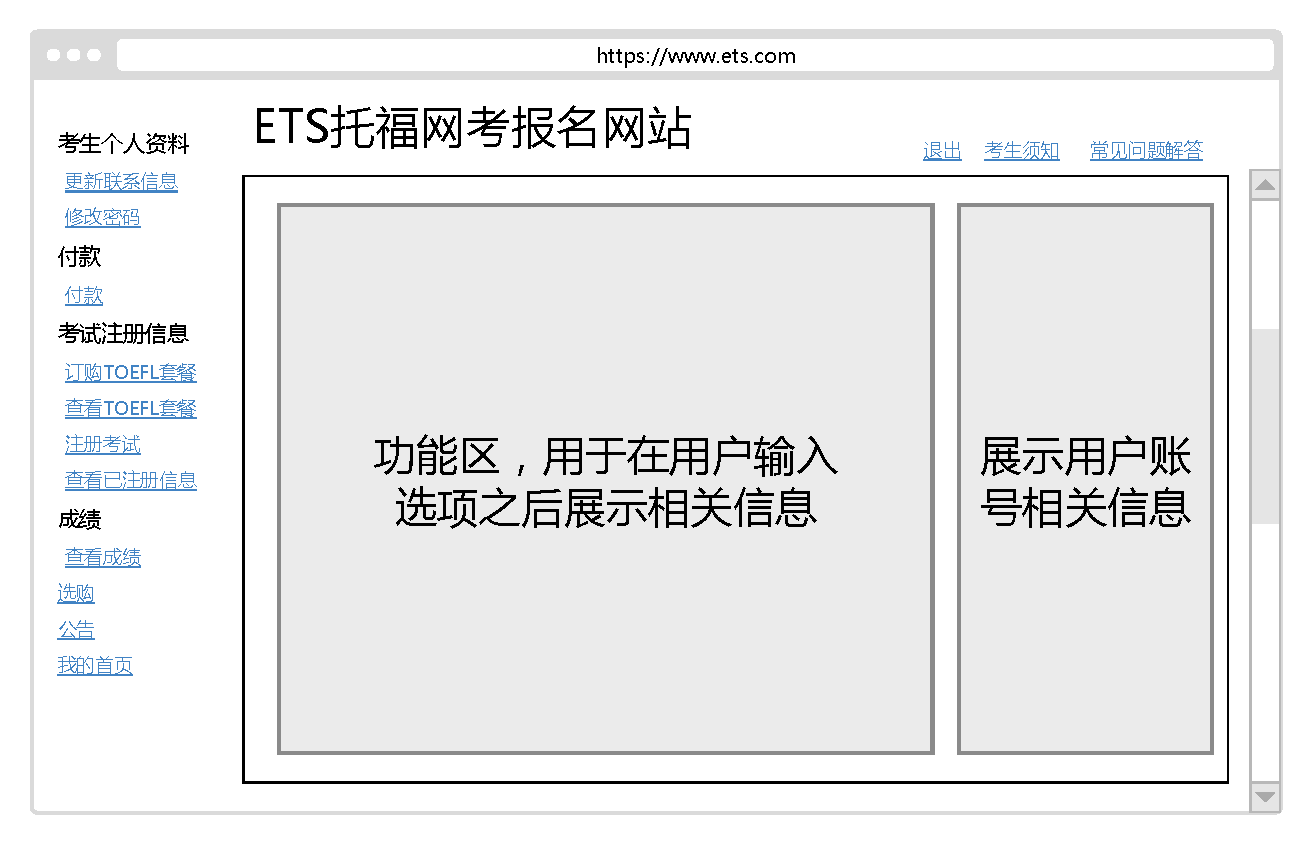
\includegraphics[width=10cm]{UI}
\caption{用户接口A}\label{fig:noted-figure}
%\note{the solid lines represent the time histogram of the spontaneous activities of an old monkey cell(gray) and a young monkey cell (black). The bin-width is 1}
\end{figure}

用户使用浏览器输入网址***.org后进入登录界面。输入ID和密码即可登录。在登录框下部提供两个按键“新用户注册”和“密码找回”。

用户点击“新用户注册”按键后,进入注册界面,其中包括各个文本框与下拉框供用户输入信息,所需输入的信息已在3.1节详细说明。

用户点击“密码找回”按键后,进入验证界面,可以选择邮箱验证或手机验证。通过注册时所填的邮箱或手机可以得到验证码,用户输入正确的验证码后,可以设置新密码。

当用户成功登录后,将进入个人中心界面,其中提供了各个功能板块,每个里面包括了一组相似功能的按键。

1、个人资料:提供“更新联系信息”和“修改密码”的按键;
	
2、考试记录:提供“考位查询”、“全年考试时间与地点查询”、“注册考试”、“查看已注册考试”、“查看成绩”的按键;

3、余额:提供“预付款”的按键。

B. 对于试题管理系统的用户接口说明如下,这一部分对应于功能需求中题库维护、试题成型和试卷批改的部分:

\begin{figure}[ht]
\centering
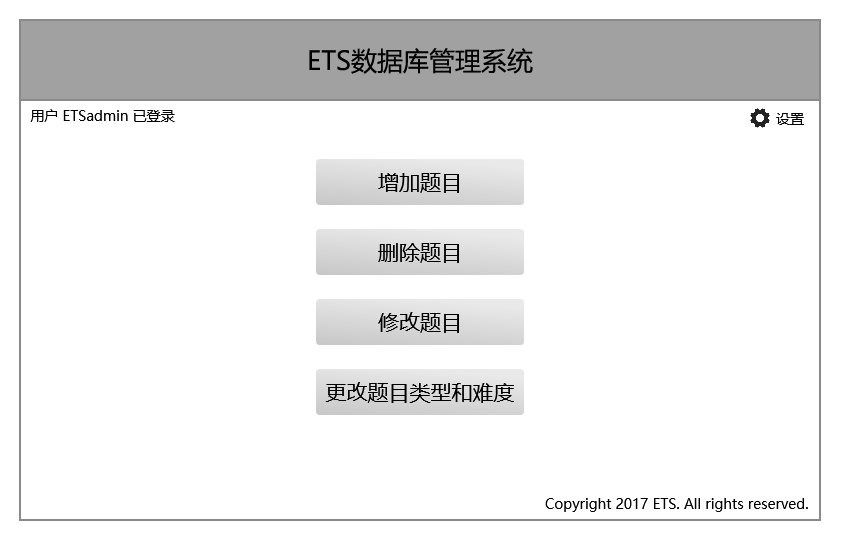
\includegraphics[width=10cm]{UI2.png}
\caption{用户接口B1}\label{fig:noted-figure}
%\note{the solid lines represent the time histogram of the spontaneous activities of an old monkey cell(gray) and a young monkey cell (black). The bin-width is 1}
\end{figure}

\begin{figure}[ht]
\centering
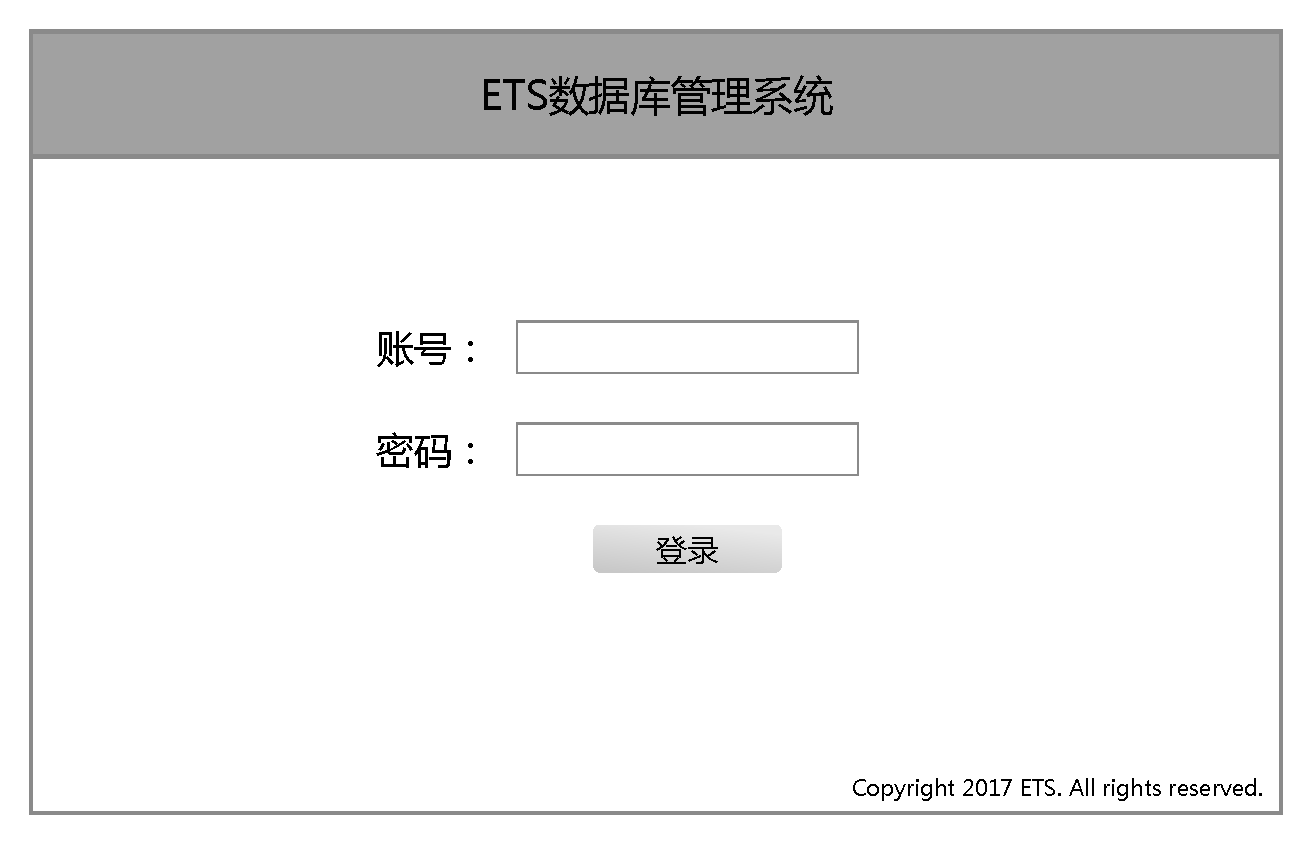
\includegraphics[width=10cm]{UI2-2}
\caption{用户接口B2}\label{fig:noted-figure}
%\note{the solid lines represent the time histogram of the spontaneous activities of an old monkey cell(gray) and a young monkey cell (black). The bin-width is 1}
\end{figure}

管理人员在服务器上运行指定的应用程序后进入登录界面,显示输入框要求输入账户和密码;登录成功后进入主界面,主界面的中央显示主菜单,菜单的选项同3.1中的说明相对应;右下角显示设置字样,点击后将能够查看设置并且进行修改。用户选择任意选项之后,主界面将按照3.1中的功能需求所对应的部分列出具体选项以及显示内容。

C. 对于考试系统的用户接口说明如下,这一部分对应于功能需求中试卷分发及测试的部分:

\begin{figure}[ht]
\centering
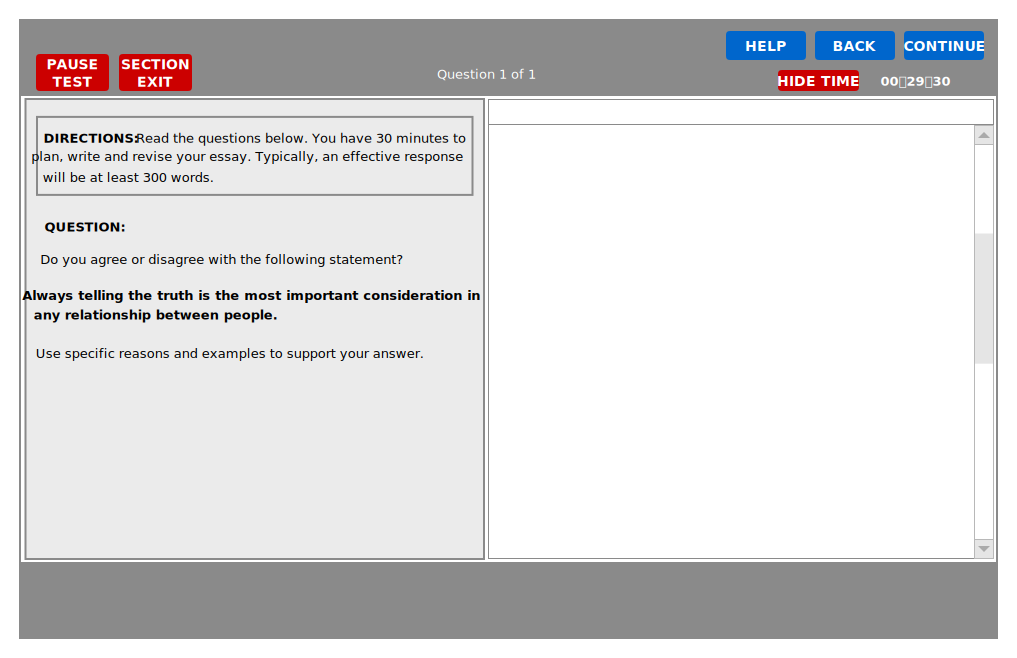
\includegraphics[width=15cm]{ETSwriting}
\caption{用户接口C1}\label{fig:noted-figure}
%\note{the solid lines represent the time histogram of the spontaneous activities of an old monkey cell(gray) and a young monkey cell (black). The bin-width is 1}
\end{figure}

\begin{figure}[ht]
\centering
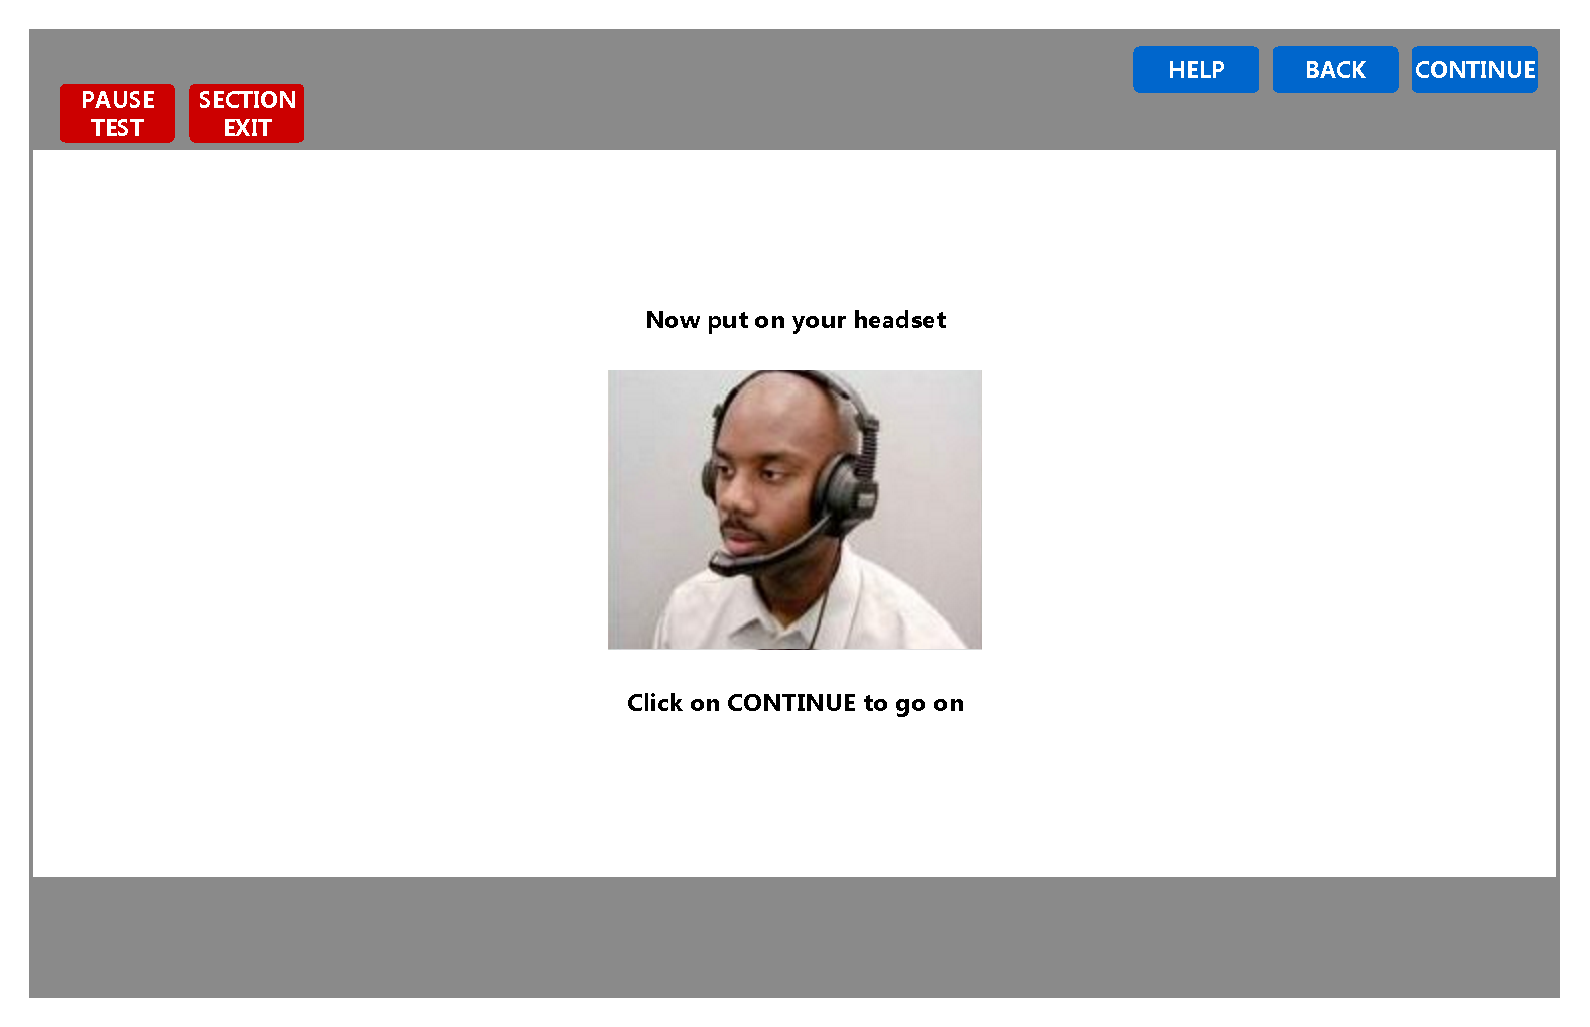
\includegraphics[width=15cm]{ETSlistening}
\caption{用户接口C2}\label{fig:noted-figure}
%\note{the solid lines represent the time histogram of the spontaneous activities of an old monkey cell(gray) and a young monkey cell (black). The bin-width is 1}
\end{figure}

用户将在考场给定的设备上使用本系统。考试未开始时,主界面将显示输入框,提示用户输入验证信息;

用户完成验证之后,主界面将显示用户的注册信息,直至考试开始;

考试开始之后,主界面将显示题目和对应的材料。用户能够根据鼠标点击来选择题目所对应的选项;主界面右上角提供调节音量、切换至下一题、切换回上一题、确认完成本部分的按钮,用户点击之后将触发相应的动作,该动作若当前不可触发应该显示为灰色;在按钮下方实时显示当前部分所剩余的时间,并且在时间的右侧显示“隐藏时间”的按钮,用户点击之后时间将被隐藏。

另外,在展示题目时,如果该部分材料需要和题目一同出现,那么将以页面的中轴线为界,在右侧显示材料,左侧显示相应的题目。对于阅读材料,用户应当能够利用鼠标滚轮上下移动材料。只显示题目时,题目应当显示在屏幕中央。

以上三部分都应具有友好的用户界面和使用提示,使得没有系统使用基础的用户不需要经过特定的培训就可以顺利使用本系统。

\subsection{软件接口}
本系统所使用的其他软件产品有

1、服务器操作系统:Windows 2012 Server,来源为微软公司,助记符为Windows Server。该软件接口的目的是为系统提供与机器交互的基础服务;

2、数据库管理系统:Oracle Database 12c 企业版,助记符Oracle数据库,来源为Oracle公司;

3、浏览器:Chrome Windows 7/8/8.1/10 32/64bit桌面版,助记符Chrome,来源为Google公司;以及Internet Explorer 10桌面版,助记符IE,来源为微软公司;

4、客户机操作系统:Windows 7 professional, 来源为微软公司,助记符为win7。该软件接口的目的是为系统提供与机器交互的基础服务。

软件的详细使用方法可以参见各软件提供公司所编写的相关文档。

\subsection{硬件接口}
A. 对于用户注册与管理系统, 该系统可以运行在支持浏览器的任意桌面计算机或PC上;

B. 对于试题管理系统,该系统可以运行在x64或者IA架构的服务器上;

C. 对于考试系统,该系统可以运行在支持IE浏览器的Windows 7/8/8.1/10系统上。

\subsection{通讯接口}
对于本系统中可以运行在浏览器上的部分,通讯协议可以参考各浏览器的软件开发文档以及对应的通讯协议标准定义,例如RFC 2818(HTTPS)等;

对于本系统中运行在服务器上的部分,通讯协议可以参考Oracle或者Microsoft公司所提供的相关文档;

对于本系统中考场测试终端和服务器进行通信的部分,可能需要使用VPN或者其他技术来确保数据的安全性,这一部分可以参照相关加密技术的标准文档以及专有网络构建所需要使用的协议及相关说明。
